\documentclass[12pt]{article}


\usepackage{amssymb}
\usepackage{amsmath}
\usepackage{fullpage}
\usepackage{epsfig}
\usepackage{epstopdf, hyperref, xcolor}
\everymath{\displaystyle}



\begin{document}

\begin{center}
\underline{\LARGE{Trigonometric Integral}}
\end{center}

\noindent SUGGESTED REFERENCE MATERIAL:

\bigskip

\noindent As you work through the problems listed below, you should reference Chapter 7.3 of the recommended textbook (or the equivalent chapter in your alternative textbook/online resource) and your lecture notes.

\bigskip

\noindent EXPECTED SKILLS:

\begin{itemize}

\item Know antiderivatives for all six elementary trigonometric functions. 

\item Be able to evaluate integrals that involve powers of sine, cosine, tangent, and secant by using appropriate trigonometric identities.

\end{itemize}

\noindent PRACTICE PROBLEMS:

\medskip

\begin{enumerate}

\item Fill in the following table

\begin{center}
\begin{tabular}{c|c}
$\int{\sin{x}}\,dx=$&\hspace{1 cm}\includegraphics[scale=0.5]{start.pdf}
{{$-\cos{x}+C$}}
\includegraphics[scale=0.5]{end.pdf}
 \hspace{1 cm}\\
\hline
$\int{\cos{x}}\,dx=$&\hspace{1 cm}\includegraphics[scale=0.5]{start.pdf}
{{$\sin{x}+C$}}
\includegraphics[scale=0.5]{end.pdf}
 \hspace{1 cm}\\
\hline
$\int{\tan{x}}\,dx=$&\hspace{1 cm}\includegraphics[scale=0.5]{start.pdf}
{{$\ln{|\sec{x}|}+C$}}
\includegraphics[scale=0.5]{end.pdf}
 \hspace{1 cm}\\
\hline
$\int{\cot{x}}\,dx=$&\hspace{1 cm}\includegraphics[scale=0.5]{start.pdf}
{{$\ln{|\sin{x}|}+C$}}
\includegraphics[scale=0.5]{end.pdf}
 \hspace{1 cm}\\
\hline
$\int{\sec{x}}\,dx=$&\hspace{1 cm}\includegraphics[scale=0.5]{start.pdf}
{{$\ln{|\sec{x}+\tan{x}|}+C$}}
\includegraphics[scale=0.5]{end.pdf}
 \hspace{1 cm}\\
\hline
$\int{\csc{x}}\,dx=$&\hspace{1 cm}\includegraphics[scale=0.5]{start.pdf}
{{$-\ln{|\csc{x}+\cot{x}|}+C$}}
\includegraphics[scale=0.5]{end.pdf}
 \hspace{1 cm}\\
\end{tabular}
\end{center}

\item $\int_{\pi/4}^{\pi/3} \cot{2x}dx$ 

\includegraphics[scale=0.5]{start.pdf}
{{$\frac{1}{4}\ln{3}-\frac{1}{2}\ln{2}$}}
\includegraphics[scale=0.5]{end.pdf}


\end{enumerate}

\noindent {\bf \underline{Powers of Sines \& Cosines:}  For each of the following, evaluate the given integral.}

\begin{enumerate}
\setcounter{enumi}{2}

\item $\int \sin{(x)}\cos^3{(x)}\,dx$ 

\includegraphics[scale=0.5]{start.pdf}
{{$-\frac{1}{4}\cos^4{x}+C$}}
\includegraphics[scale=0.5]{end.pdf}


\item $\int \sin^3{(x)}\cos^4{(x)}\,dx$ 

\includegraphics[scale=0.5]{start.pdf}
{{$\frac{1}{7}\cos^7{x}-\frac{1}{5}\cos^5{x}+C$}}
\includegraphics[scale=0.5]{end.pdf}


\item $\int \sqrt{\sin{x}}\cos^{3}{(x)}\,dx$

\includegraphics[scale=0.5]{start.pdf}
{{$\frac{2}{3}(\sin{x})^{3/2}-\frac{2}{7}(\sin{x})^{7/2}+C$}}
\includegraphics[scale=0.5]{end.pdf}


\item $\int \sin^2{x} \,dx$ 

\includegraphics[scale=0.5]{start.pdf}
{{$\frac{x}{2}-\frac{1}{4}\sin{(2x)}+C$}}
\includegraphics[scale=0.5]{end.pdf}


\item $\int \sin^3{(bx)}\,dx$, where $b$ is a non-zero constant

\includegraphics[scale=0.5]{start.pdf}
{{$\frac{1}{3b}\cos^3{(bx)}-\frac{1}{b}\cos{(bx)}+C$; Detailed Solution: \textcolor{blue}{\href{http://www.math.drexel.edu/classes/Calculus/resources/Math122HW/Solutions/122_15_Trig_Int_07.pdf}{Here}}}}
\includegraphics[scale=0.5]{end.pdf}


\item $\int \sin^2{x}\cos^2{x}\,dx$ 

\includegraphics[scale=0.5]{start.pdf}
{{$\frac{x}{8}-\frac{1}{32}\sin{(4x)}+C$}}
\includegraphics[scale=0.5]{end.pdf}


\item $\int_{\pi/4}^{\pi/2} \cos^3{x}\,dx$ 

\includegraphics[scale=0.5]{start.pdf}
{{$\frac{2}{3}-\frac{5\sqrt{2}}{12}$}}
\includegraphics[scale=0.5]{end.pdf}


\item $\int \cos^4{5x}\,dx$

\includegraphics[scale=0.5]{start.pdf}
{{$\frac{3}{8}x+\frac{1}{20}\sin{(10x)}+\frac{1}{160}\sin{(20x)}+C$}}
\includegraphics[scale=0.5]{end.pdf}


\item Consider the trigonmetric identity $\sin{(A+B)}=\sin{A}\cos{B}+\cos{A}\sin{B}$

\begin{enumerate}

\item Use this identity to derive an identity for $\sin{(A-B)}$ in terms of $\sin{A}$, $\cos{A}$, $\sin{B}$, and $\cos{B}$.

\includegraphics[scale=0.5]{start.pdf}
{{$\sin{(A-B)}=\sin{A}\cos{B}-\cos{A}\sin{B}$}}
\includegraphics[scale=0.5]{end.pdf}


\item Use the given identity and your answer for part (a) to derive the following identity: $$\sin{A}\cos{B}=\frac{1}{2}\left[\sin{(A-B)}+\sin{(A+B)}\right]$$

\includegraphics[scale=0.5]{start.pdf}
{{{1\linewidth}{Adding the given identity to the identity from part (a) and then dividing both sides by 2 yields the desired result.}}}
\includegraphics[scale=0.5]{end.pdf}


\end{enumerate}

\item Consider the trigonmetric identity $\cos{(A+B)}=\cos{A}\cos{B}-\sin{A}\sin{B}$

\begin{enumerate}

\item Use this identity to derive an identity for $\cos{(A-B)}$ in terms of $\sin{A}$, $\cos{A}$, $\sin{B}$, and $\cos{B}$.

\includegraphics[scale=0.5]{start.pdf}
{{$\cos{(A-B)}=\cos{A}\cos{B}+\sin{A}\sin{B}$}}
\includegraphics[scale=0.5]{end.pdf}


\item Use the given identity and your answer for part (a) to derive the following identity: $$\cos{A}\cos{B}=\frac{1}{2}\left[\cos{(A-B)}+\cos{(A+B)}\right]$$

\includegraphics[scale=0.5]{start.pdf}
{{{1\linewidth}{Adding the given identity to the identity from part (a) and then dividing both sides by 2 yields the desired result.}}}
\includegraphics[scale=0.5]{end.pdf}


\item Use the given identity and your answer for part (a) to derive the following identity: $$\sin{A}\sin{B}=\frac{1}{2}\left[\cos{(A-B)}-\cos{(A+B)}\right]$$

\includegraphics[scale=0.5]{start.pdf}
{{{1\linewidth}{Subtracting the given identity from the identity from part (a) and then dividing both sides by 2 yields the desired result.}}}
\includegraphics[scale=0.5]{end.pdf}


\end{enumerate}

\end{enumerate}

\noindent {\bf For problems 13-16, use an appropriate identity from problem 11 or 12 to evaluate the given integral.}

\begin{enumerate}
\setcounter{enumi}{12}

\item $\int \sin{(2x)}\cos{\left(\frac{x}{2}\right)}\,dx$ 

\includegraphics[scale=0.5]{start.pdf}
{{$-\frac{1}{5}\cos{\left(\frac{5x}{2}\right)}-\frac{1}{3}\cos{\left(\frac{3x}{2}\right)}+C$}}
\includegraphics[scale=0.5]{end.pdf}


\item $\int \cos{(3x)}\cos{(4x)}\,dx$ 

\includegraphics[scale=0.5]{start.pdf}
{{$\frac{1}{2}\sin{x}+\frac{1}{14}\sin{(7x)}+C$}}
\includegraphics[scale=0.5]{end.pdf}


\item $\int \sin{(5x)}\cos{(2x)}\,dx$ 

\includegraphics[scale=0.5]{start.pdf}
{{$-\frac{1}{6}\cos{(3x)}-\frac{1}{14}\cos{(7x)}+C$}}
\includegraphics[scale=0.5]{end.pdf}


\newpage

\item The graph of $f(x)=\sin{2x}\sin{5x}$ on the interval $[-\pi,\pi]$ is shown below.

\begin{center}
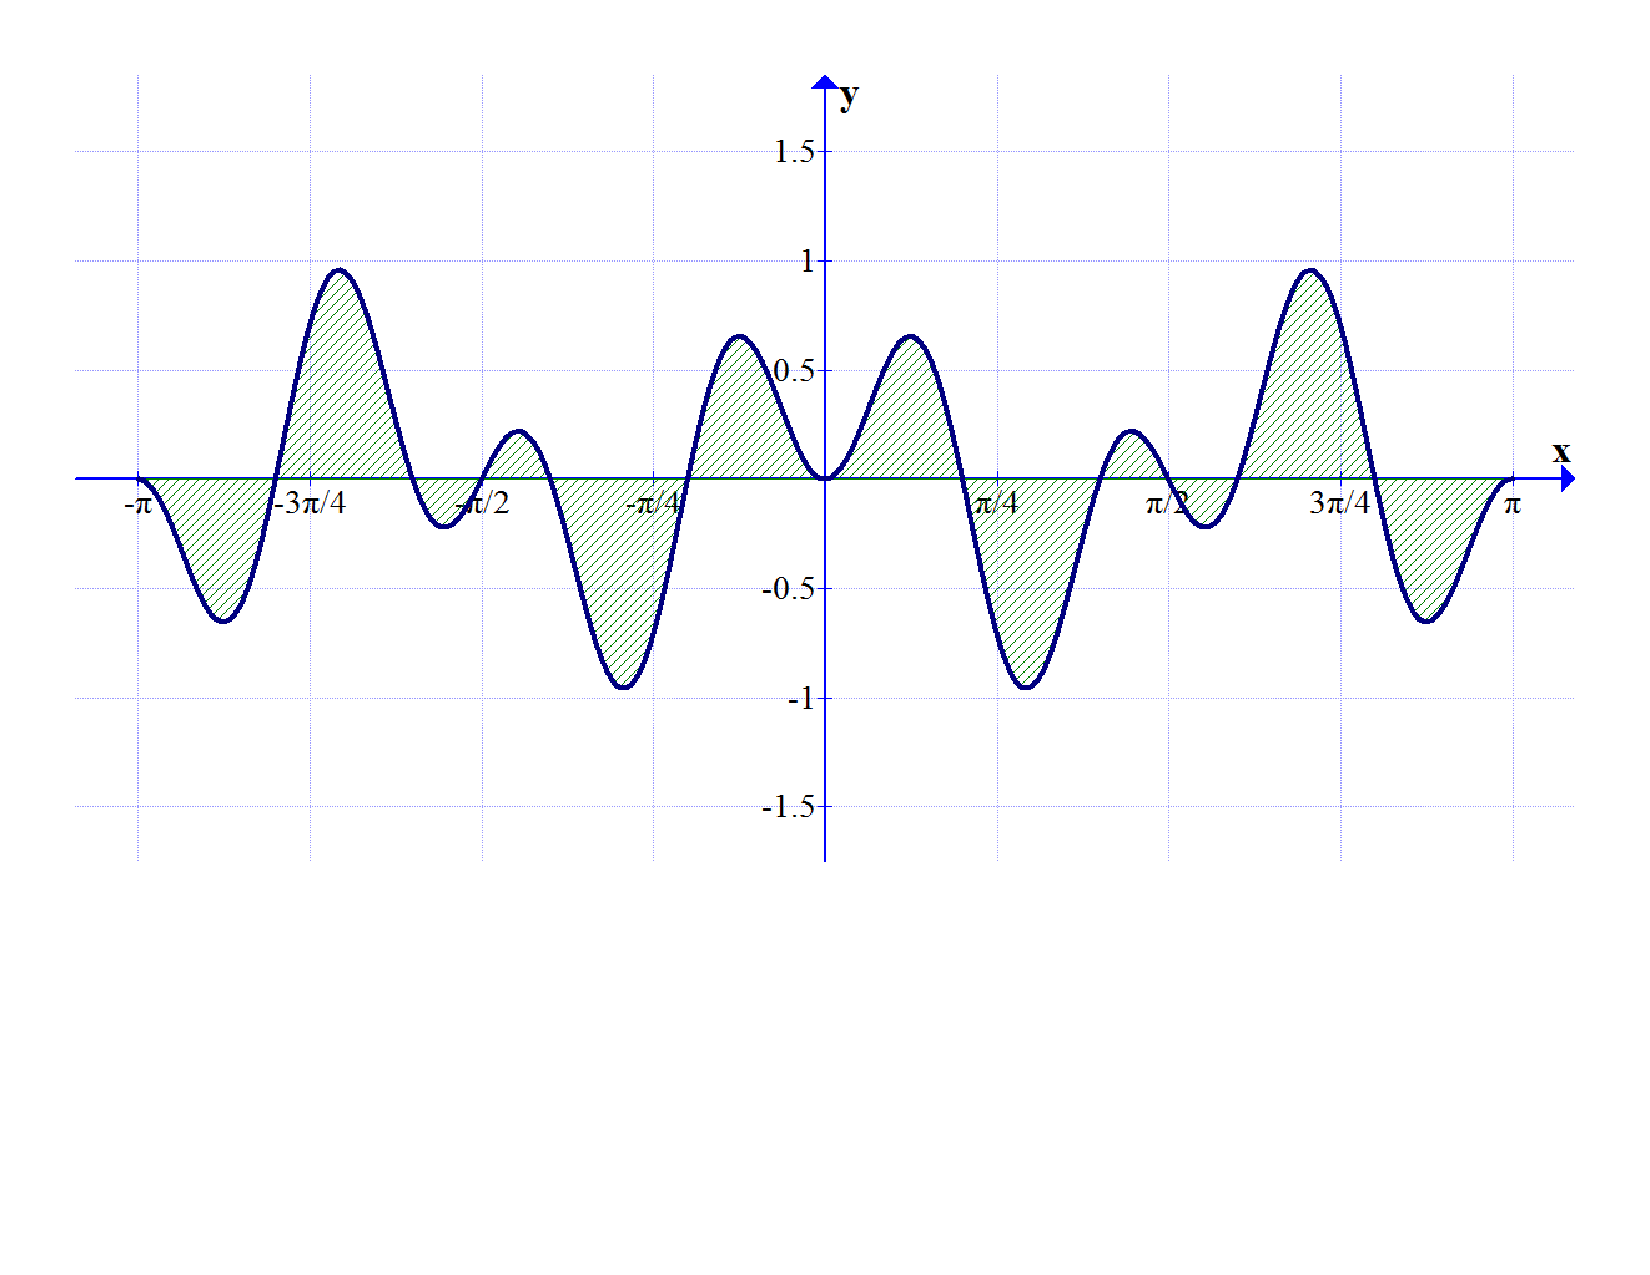
\includegraphics[scale=0.3]{graph.pdf}
\end{center}

Compute the net signed area between the graph of $f(x)$ and the $x$-axis on the interval $[-\pi,\pi]$

\includegraphics[scale=0.5]{start.pdf}
{{0}}
\includegraphics[scale=0.5]{end.pdf}


\end{enumerate}

\noindent {\bf \underline{Powers of Tangents \& Secants:}  For each of the following, evaluate the given integral.}

\begin{enumerate}
\setcounter{enumi}{16}

\item $\int \tan^2{3x}\,dx$ 

\includegraphics[scale=0.5]{start.pdf}
{{$-x+\frac{1}{3}\tan{(3x)}+C$}}
\includegraphics[scale=0.5]{end.pdf}


\item $\int_0^{\pi/4} \tan^{3}{(x)}\sec^3{(x)}\,dx$  

\includegraphics[scale=0.5]{start.pdf}
{{$\frac{2}{15}\left(1+\sqrt{2}\right)$}}
\includegraphics[scale=0.5]{end.pdf}


\item $\int \tan{(x)}\sec^3{(x)}dx$ 

\includegraphics[scale=0.5]{start.pdf}
{{$\frac{1}{3}\sec^3{x}+C$}}
\includegraphics[scale=0.5]{end.pdf}


\item $\int \tan^3{(x)}\sec^4{(x)\,}dx$ 

\includegraphics[scale=0.5]{start.pdf}
{{$\frac{1}{6}\tan^6{x}+\frac{1}{4}\tan^{4}{x}+C$}}
\includegraphics[scale=0.5]{end.pdf}


\item $\int \tan^5{(2x)}\sec^2{(2x)}\,dx$ 

\includegraphics[scale=0.5]{start.pdf}
{{$\frac{1}{12}\tan^6{(2x)}+C$}}
\includegraphics[scale=0.5]{end.pdf}


\item $\int \tan{(x)}\sec^{5/2}{(x)}\,dx$ 

\includegraphics[scale=0.5]{start.pdf}
{{$\frac{2}{5}\sec^{5/2}{x}+C$; Detailed Solution: \textcolor{blue}{\href{http://www.math.drexel.edu/classes/Calculus/resources/Math122HW/Solutions/122_15_Trig_Int_22.pdf}{Here}}}}
\includegraphics[scale=0.5]{end.pdf}


\item $\int \sec^{4}{x}\,dx$ 

\includegraphics[scale=0.5]{start.pdf}
{{$\frac{1}{3}\tan^3{x}+\tan{x}+C$}}
\includegraphics[scale=0.5]{end.pdf}


\item Consider $\int_{\pi/2}^\pi \sec{x} \,dx$

\begin{enumerate}

\item Explain why this integral is improper.

\includegraphics[scale=0.5]{start.pdf}
{{{1\linewidth}{The integral is improper because $\sec{x}$ has an infinite discontinuity at $x=\frac{\pi}{2}$ which is the lower limit of integration.}}}
\includegraphics[scale=0.5]{end.pdf}


\item Evaluate the given integral.  If it diverges, explain why.

\includegraphics[scale=0.5]{start.pdf}
{{The integral diverges because $\int_{\pi/2}^{\pi} \sec{x} \,dx = -\infty$}}
\includegraphics[scale=0.5]{end.pdf}


\end{enumerate}

\item \begin{enumerate}

\item Use integration by parts to evaluate $\int \sec^{3}{(x)}\,dx$.  (Hint: $\sec^3{x}=\sec^2{x}\sec{x}$ and $\tan^2{x}=\sec^2{x}-1$)

\includegraphics[scale=0.5]{start.pdf}
{{$\frac{1}{2}\sec{(x)}\tan{(x)}+\frac{1}{2}\ln{|\sec{x}+\tan{x}|}+C$}}
\includegraphics[scale=0.5]{end.pdf}


\item Use part (a) to evaluate $\int \tan^{2}{(x)}\sec{(x)}\,dx$

\includegraphics[scale=0.5]{start.pdf}
{{$\frac{1}{2}\sec{(x)}\tan{(x)}-\frac{1}{2}\ln{|\sec{x}+\tan{x}|}+C$}}
\includegraphics[scale=0.5]{end.pdf}


\end{enumerate}

\item Let $R$ be the region bounded between the graphs of $y=\sin{x}$ and $y=\cos{x}$ on the interval $\left[\frac{\pi}{4},\frac{\pi}{2}\right]$.

\begin{enumerate}

\item Compute the area of $R$.

\includegraphics[scale=0.5]{start.pdf}
{{$\sqrt{2}-1$}}
\includegraphics[scale=0.5]{end.pdf}


\item Compute the volume of the solid which results from revolving $R$ around the $x$-axis.

\includegraphics[scale=0.5]{start.pdf}
{{$\frac{\pi}{2}$}}
\includegraphics[scale=0.5]{end.pdf}


\end{enumerate}

\item Find the length of the curve $y=\ln{(\sin{x})}$ on the interval $\left[\frac{\pi}{4},\frac{3\pi}{4}\right]$.

\includegraphics[scale=0.5]{start.pdf}
{{$2\ln{\left(2+\sqrt{2}\right)}-\ln{2}$; Detailed Solution: \textcolor{blue}{\href{http://www.math.drexel.edu/classes/Calculus/resources/Math122HW/Solutions/122_15_Trig_Int_27.pdf}{Here}}}}
\includegraphics[scale=0.5]{end.pdf}


\end{enumerate}

\end{document}